\section*{Exercice 5 : Unit� � virgule flottante (5.5 points)}

{\bf x87 FPU :}

L'unit\'e \`a virgule flottante (FPU) du Pentium, la x87 FPU, est un
composant int\'egr\'e au microprocesseur et offrant le support des nombres
flottants IEEE 754.

La FPU contient les registres suivants :

\begin{itemize}
\item
  Status Register : contient les flags (Z, N\ldots)
\item
  Control Register : contient le masque d'exception
\item
  Tag Word : indique l'�tat des registres R0-R7
\item
  Instruction Pointer : pointeur vers la derni�re instruction
  flottante ex�cut�e
\item
  Instruction Opcode : opcode de la derni�re instruction flottante
  ex�cut�e
\item
  Data Pointer : pointeur vers la derni�re op�rande charg�e en
  m�moire
\item
  R0-R7 : huit registres de calcul (aussi appel�s ST(0)-ST(7))
\end{itemize}

Les instructions suivantes (sous forme de macros) manipulent
le contexte de la FPU :

\begin{itemize}
\item
  \verb|FSAVE(ptr)| : sauvegarde le contexte FPU � l'adresse
  \emph{ptr}
\item
  \verb|FRSTOR(ptr)| : restaure le contexte FPU depuis l'adresse
  \emph{ptr}
\end{itemize}

Lorsque le flag TS du registre CR0 est � 1 et qu'une instruction
flottante est ex�cut�e, une exception 7 (Device Not Available) est
lev�e. Le flag TS est mis � 0 par la macro CLTS() ou mis � 1 par
STS().

Dans l'exercice qui suit, vous utiliserez ce m�canisme
d'exception pour effectuer les changements de contexte uniquement au
moment opportun.

\begin{description}
\item {\bf Impl�mentation du changement de contexte pour la FPU}

\begin{enumerate}
\item
  Quatre threads tournent sur notre syst�me : T1, T2, T3 et T4 sont
  ex�cut�s l'un apr\`es l'autre (Round-Robin).

  Les threads T1, T2 et T4 effectuent des calculs flottants.

  \`A partir du sch�ma ci-dessous, identifiez � quels instants vous
  allez devoir changer le contexte FPU.

  \begin{center}
    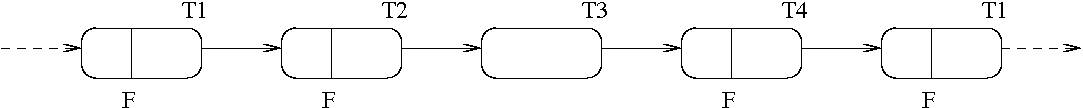
\includegraphics[width=\linewidth]{figures/cs-fpu}
  \end{center}

  D\'eduisez-en la valeur du flag TS au fil de l'ex�cution de chacun des
  threads.

\item
  La structure permettant de stocker le contexte FPU vous est
  donn�e. Elle se nomme \emph{t\_x87\_context}. Elle contient tous les
  registres cit�s plus haut. Ne vous int\'eressez pas au d\'etail de son contenu,
  mais sachez que la structure est compatible avec \verb|FSAVE| et \verb|FRSTOR|.

  Dans quel objet kaneton allez-vous stocker le contexte FPU d'un
  thread ? Dans quelle fonction de l'interface kaneton allez-vous
  initialiser ce contexte ?

  \textbf{Dans la suite de l'excercice, consid\'erez que les
  structures de contexte FPU sont correctement remplies.}
\item
  \'Ecrivez le code du gestionnaire d'interruption Device Not
  Available. C'est bien evidemment dans ce dernier que vous devez
  �changer les contextes FPU.

  Indiquez � quel endroit du code (aussi bien celui que vous venez
  d'�crire que celui des autres fonctions du scheduler) vous devez
  mettre � jour TS.

\end{enumerate}
\end{description}
